\documentclass[final, oneside, a4paper, 11pt, pdftex, english]{scrreprt}

\usepackage{babel}
\usepackage[utf8]{inputenc}
\usepackage[T1]{fontenc}
\usepackage{lmodern}

\usepackage{tikz}
\usepackage{pgf-umlcd}

\usepackage[hidelinks]{hyperref}

%\pagestyle{headings}
%\graphicspath{images}
%\raggedbottom

\newlength{\umlwidth}
\setlength{\umlwidth}{12cm}

\newcommand{\todo}[1]{\noindent\framebox[\linewidth]{\parbox{\linewidth}{\textbf{TODO:}\\#1}}}

\begin{document}

\title{pyMolDyn}
\author{Fabian Beule, David Knodt}
\date{\today}
\maketitle

\tableofcontents

%\chapter{Introduction}

\chapter{Class description}
\section{Data}

\subsection{Input data}
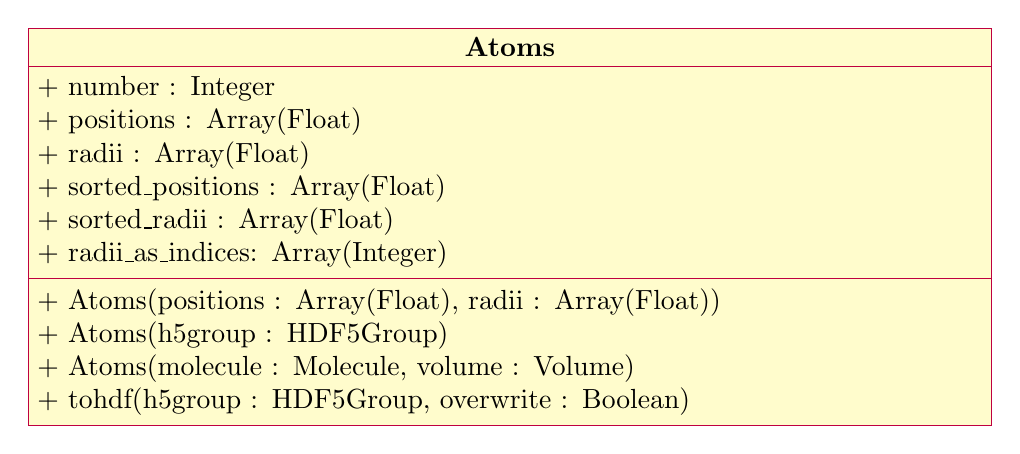
\begin{tikzpicture}
    \begin{class}[text width=\umlwidth]{Atoms}{0, 0}
        \attribute{+ number : Integer}
        \attribute{+ positions : Array(Float)}
        \attribute{+ radii : Array(Float)}
        \attribute{+ sorted\_positions : Array(Float)}
        \attribute{+ sorted\_radii : Array(Float)}
        \attribute{+ radii\_as\_indices: Array(Integer)}

        \operation{+ Atoms(positions : Array(Float), radii : Array(Float))}
        \operation{+ Atoms(h5group : HDF5Group)}
        \operation{+ Atoms(molecule : Molecule, volume : Volume)}
        \operation{+ tohdf(h5group : HDF5Group, overwrite : Boolean)}
    \end{class}
\end{tikzpicture}

\subsection{Calculation results}
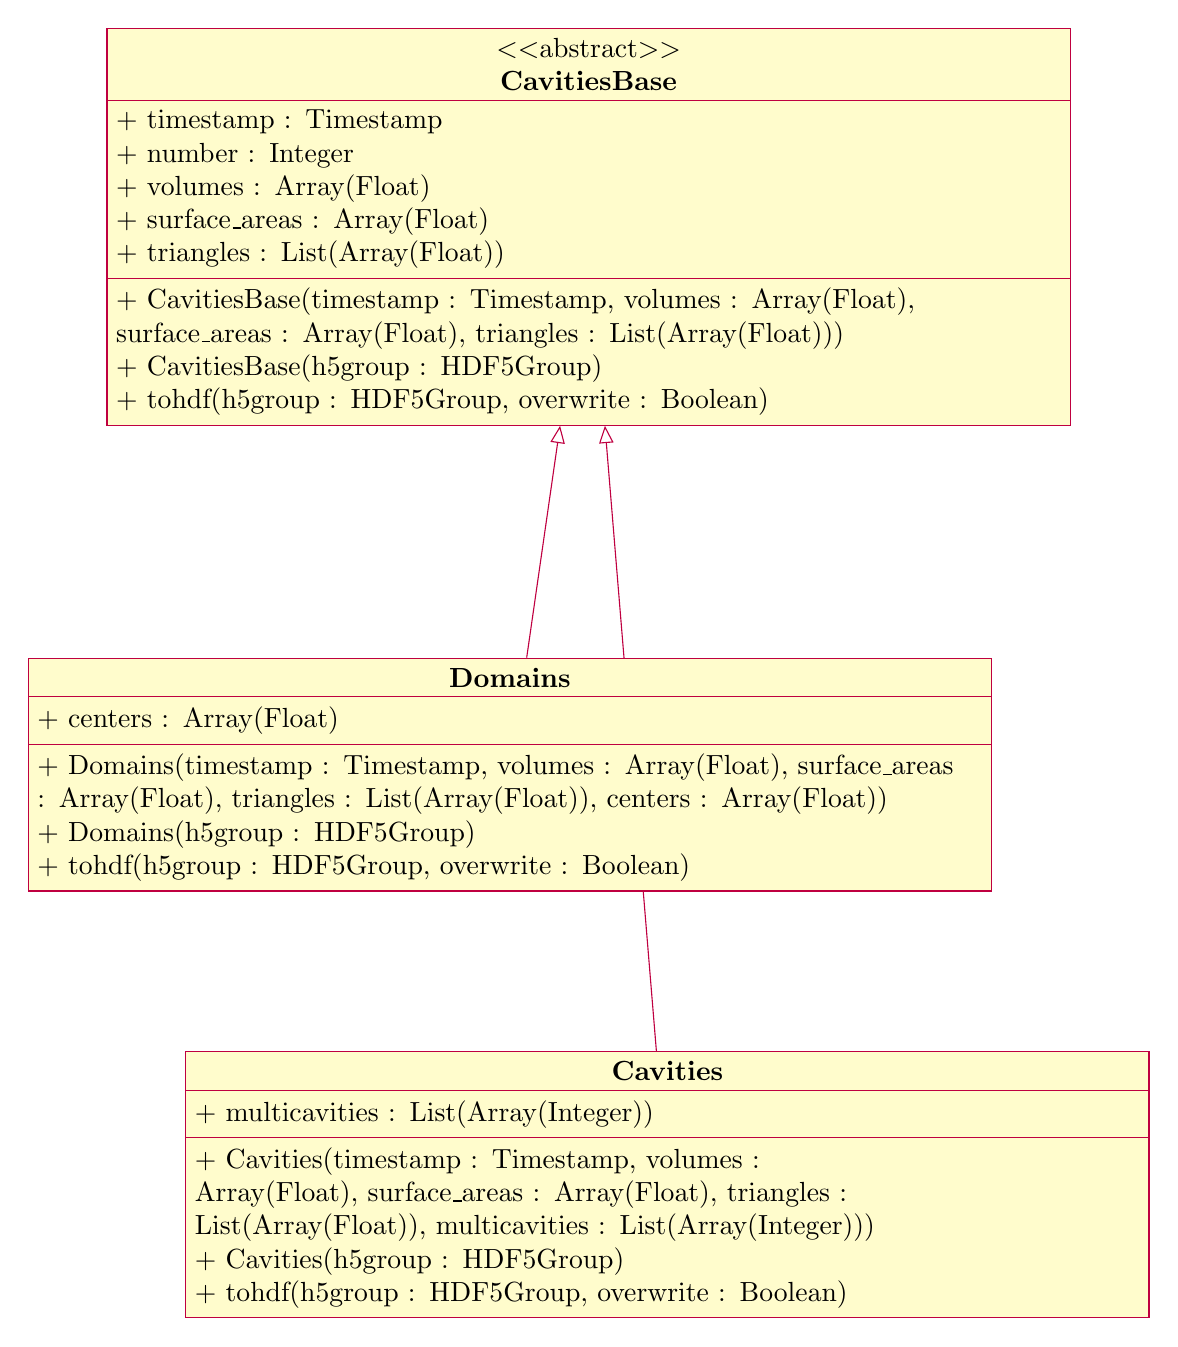
\begin{tikzpicture}
    \begin{abstractclass}[text width=\umlwidth]{CavitiesBase}{0, 0}
        \attribute{+ timestamp : Timestamp}
        \attribute{+ number : Integer}
        \attribute{+ volumes : Array(Float)}
        \attribute{+ surface\_areas : Array(Float)}
        \attribute{+ triangles : List(Array(Float))}

        \operation{+ CavitiesBase(timestamp : Timestamp, volumes : Array(Float), surface\_areas : Array(Float), triangles : List(Array(Float)))}
        \operation{+ CavitiesBase(h5group : HDF5Group)}
        \operation{+ tohdf(h5group : HDF5Group, overwrite : Boolean)}
    \end{abstractclass}

    \begin{class}[text width=\umlwidth]{Domains}{-1, -8}
        \inherit{CavitiesBase}
        
        \attribute{+ centers : Array(Float)}

        \operation{+ Domains(timestamp : Timestamp, volumes : Array(Float), surface\_areas : Array(Float), triangles : List(Array(Float)), centers : Array(Float))}
        \operation{+ Domains(h5group : HDF5Group)}
        \operation{+ tohdf(h5group : HDF5Group, overwrite : Boolean)}
    \end{class}

    \begin{class}[text width=\umlwidth]{Cavities}{1, -13}
        \inherit{CavitiesBase}

        \attribute{+ multicavities : List(Array(Integer))}

        \operation{+ Cavities(timestamp : Timestamp, volumes : Array(Float), surface\_areas : Array(Float), triangles : List(Array(Float)), multicavities : List(Array(Integer)))}
        \operation{+ Cavities(h5group : HDF5Group)}
        \operation{+ tohdf(h5group : HDF5Group, overwrite : Boolean)}
    \end{class}
\end{tikzpicture}

\noindent
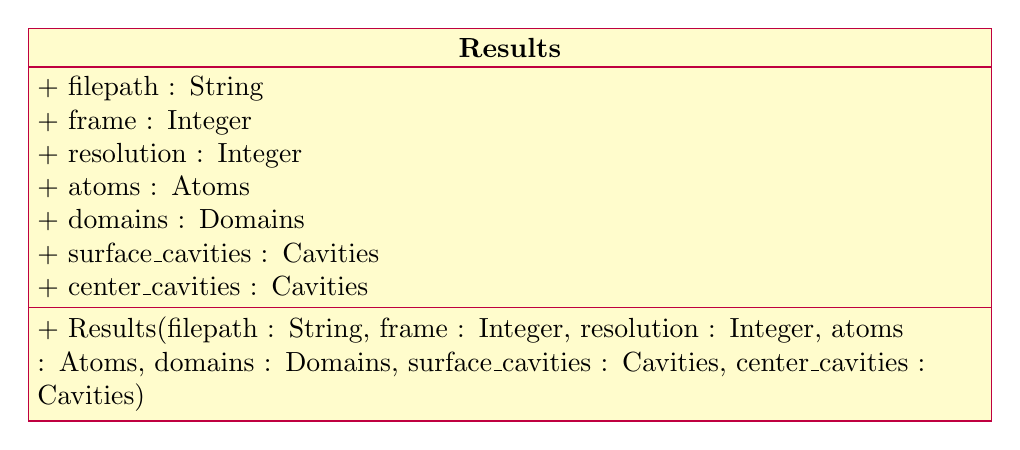
\begin{tikzpicture}
    \begin{class}[text width=\umlwidth]{Results}{0, 0}
        \attribute{+ filepath : String}
        \attribute{+ frame : Integer}
        \attribute{+ resolution : Integer}
        \attribute{+ atoms : Atoms}
        \attribute{+ domains : Domains}
        \attribute{+ surface\_cavities : Cavities}
        \attribute{+ center\_cavities : Cavities}

        \operation{+ Results(filepath : String, frame : Integer, resolution : Integer, atoms : Atoms, domains : Domains, surface\_cavities : Cavities, center\_cavities : Cavities)}
    \end{class}
\end{tikzpicture}

\subsection{Meta data}
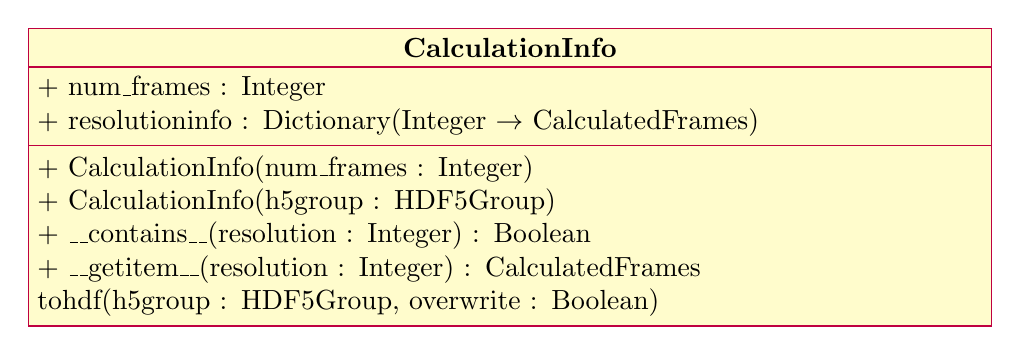
\begin{tikzpicture}
    \begin{class}[text width=\umlwidth]{CalculationInfo}{0, 0}
        \attribute{+ num\_frames : Integer}
        \attribute{+ resolutioninfo : Dictionary(Integer $\rightarrow$ CalculatedFrames)}

        \operation{+ CalculationInfo(num\_frames : Integer)}
        \operation{+ CalculationInfo(h5group : HDF5Group)}
        \operation{+ \_\_contains\_\_(resolution : Integer) : Boolean}
        \operation{+ \_\_getitem\_\_(resolution : Integer) : CalculatedFrames}
        \operation{tohdf(h5group : HDF5Group, overwrite : Boolean)}
    \end{class}
\end{tikzpicture}

\noindent
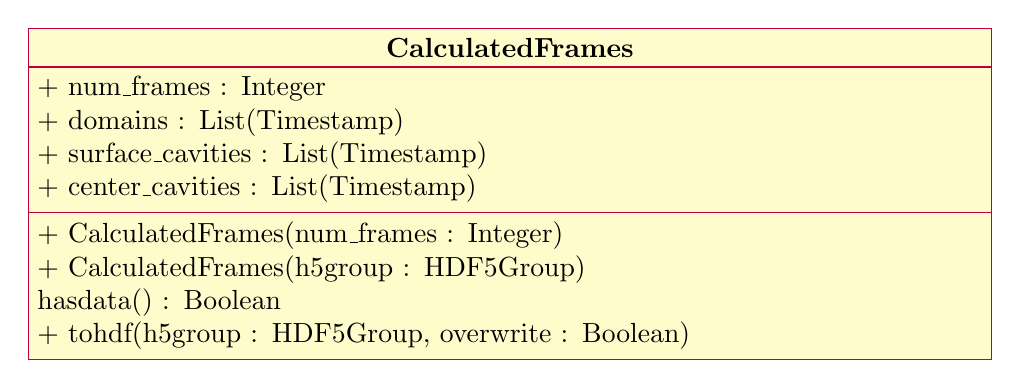
\begin{tikzpicture}
    \begin{class}[text width=\umlwidth]{CalculatedFrames}{0, 0}
        \attribute{+ num\_frames : Integer}
        \attribute{+ domains : List(Timestamp)}
        \attribute{+ surface\_cavities : List(Timestamp)}
        \attribute{+ center\_cavities : List(Timestamp)}

        \operation{+ CalculatedFrames(num\_frames : Integer)}
        \operation{+ CalculatedFrames(h5group : HDF5Group)}
        \operation{hasdata() : Boolean}
        \operation{+ tohdf(h5group : HDF5Group, overwrite : Boolean)}
    \end{class}
\end{tikzpicture}


\section{File handling}

\subsection{Abstract file classes}
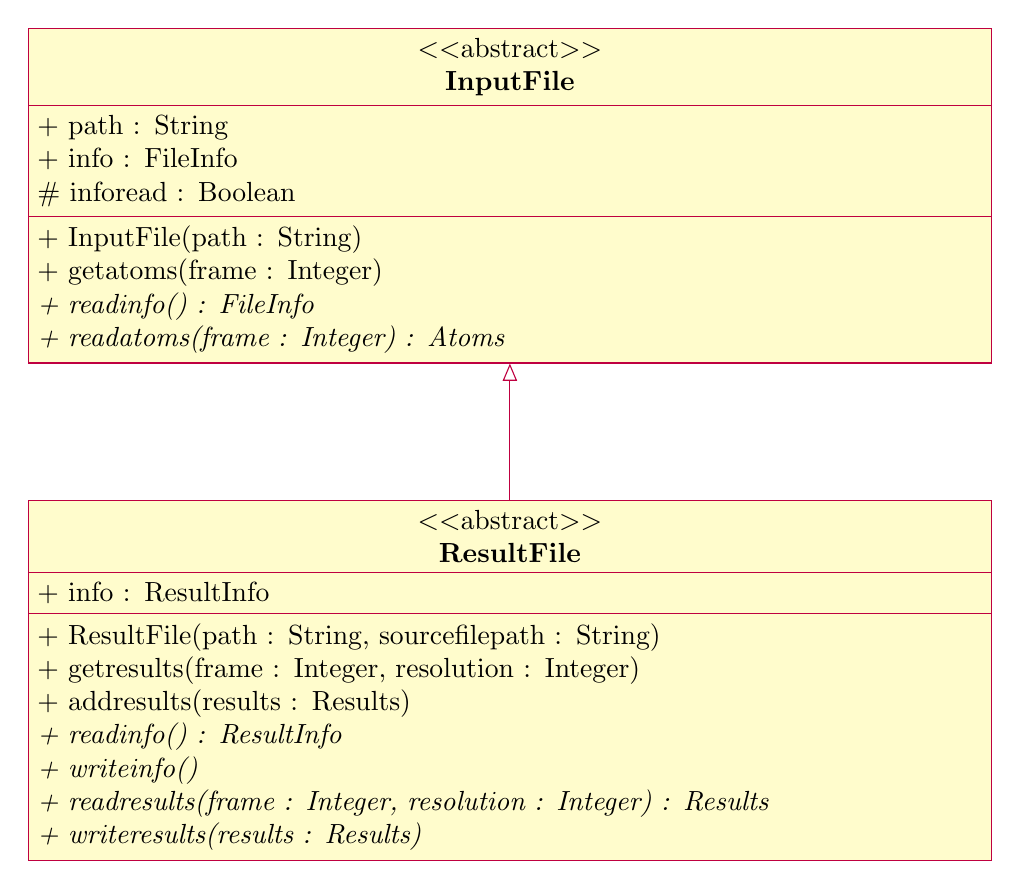
\begin{tikzpicture}
    \begin{abstractclass}[text width=\umlwidth]{InputFile}{0, 0}
        \attribute{+ path : String}
        \attribute{+ info : FileInfo}
        \attribute{\# inforead : Boolean}

        \operation{+ InputFile(path : String)}
        \operation{+ getatoms(frame : Integer)}
        \operation[0]{+ readinfo() : FileInfo}
        \operation[0]{+ readatoms(frame : Integer) : Atoms}
    \end{abstractclass}

    \begin{abstractclass}[text width=\umlwidth]{ResultFile}{0, -6}
        \inherit{InputFile}

        \attribute{+ info : ResultInfo}

        \operation{+ ResultFile(path : String, sourcefilepath : String)}
        \operation{+ getresults(frame : Integer, resolution : Integer)}
        \operation{+ addresults(results : Results)}
        \operation[0]{+ readinfo() : ResultInfo}
        \operation[0]{+ writeinfo()}
        \operation[0]{+ readresults(frame : Integer, resolution : Integer) : Results}
        \operation[0]{+ writeresults(results : Results)}
    \end{abstractclass}
\end{tikzpicture}

\todo{\texttt{ResultFile.writeresults} should take an \texttt{overwrite} parameter.}

\noindent
The implementation of \texttt{InputFile} is \texttt{XYZFile}, which reads a pybel xyz file. \texttt{HDF5File} implements \texttt{ResultFile} and handles a HDF5 file with input and result data, which can be used for caching.


\subsection{Filesystem access}
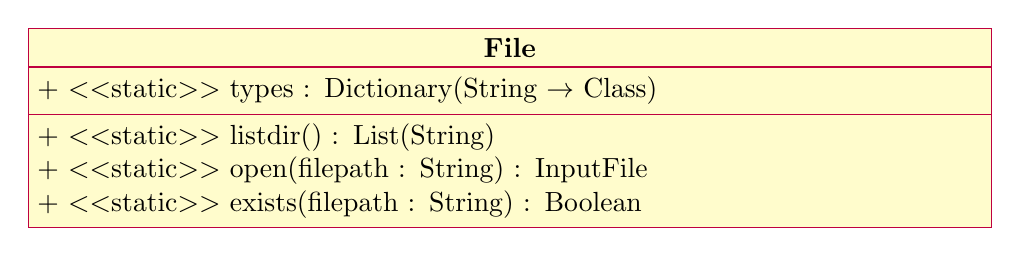
\begin{tikzpicture}
    \begin{class}[text width=\umlwidth]{File}{0, 0}
        \attribute{+ $<<$static$>>$ types : Dictionary(String $\rightarrow$ Class)}
        
        \operation{+ $<<$static$>>$ listdir() : List(String)}
        \operation{+ $<<$static$>>$ open(filepath : String) : InputFile}
        \operation{+ $<<$static$>>$ exists(filepath : String) : Boolean}
    \end{class}
\end{tikzpicture}

The \texttt{types} dictionary is used to associate filename extensions (e.\,g.\ xyz) with implementations of \texttt{InputFile}.
\texttt{open} looks up which class to use and instanciates it.

\todo{Overrideable \texttt{detectfiletype} method (flexibility),\\
unfiltered file list}


\section{Cavity and domain calculation}
\subsection{Calculation and cache lookup}
The interface to get calculation Results:\\
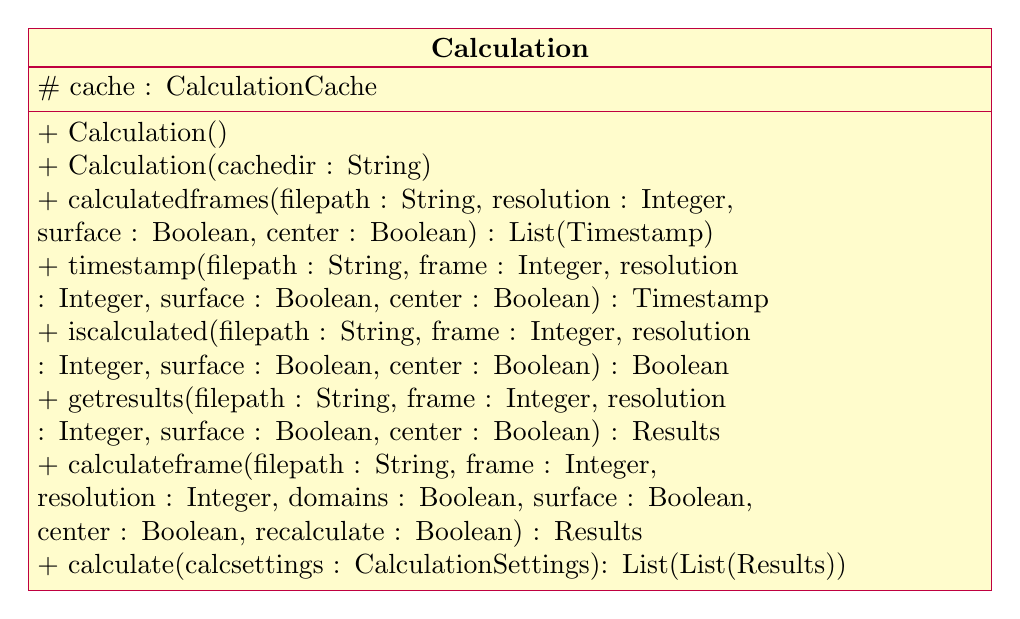
\begin{tikzpicture}
    \begin{class}[text width=\umlwidth]{Calculation}{0, 0}
        \attribute{\# cache : CalculationCache}
        
        \operation{+ Calculation()}
        \operation{+ Calculation(cachedir : String)}
        \operation{+ calculatedframes(filepath : String, resolution : Integer, surface : Boolean, center : Boolean) : List(Timestamp)}
        \operation{+ timestamp(filepath : String, frame : Integer, resolution : Integer, surface : Boolean, center : Boolean) : Timestamp}
        \operation{+ iscalculated(filepath : String, frame : Integer, resolution : Integer, surface : Boolean, center : Boolean) : Boolean}
        \operation{+ getresults(filepath : String, frame : Integer, resolution : Integer, surface : Boolean, center : Boolean) : Results}
        \operation{+ calculateframe(filepath : String, frame : Integer, resolution : Integer, domains : Boolean, surface : Boolean, center : Boolean, recalculate : Boolean) : Results}
        \operation{+ calculate(calcsettings : CalculationSettings): List(List(Results))}
    \end{class}
\end{tikzpicture}
\\
If results are cached, \texttt{getresults} returns them; if not, it returns a \texttt{Results} object with only \texttt{Atoms}.
\texttt{calculateframes} either loads results from cache or calculates them.
\texttt{calculate} returns a list with an entry for each selected file. This entry itself is a list with a \texttt{Result} for each selcted frame.

\noindent
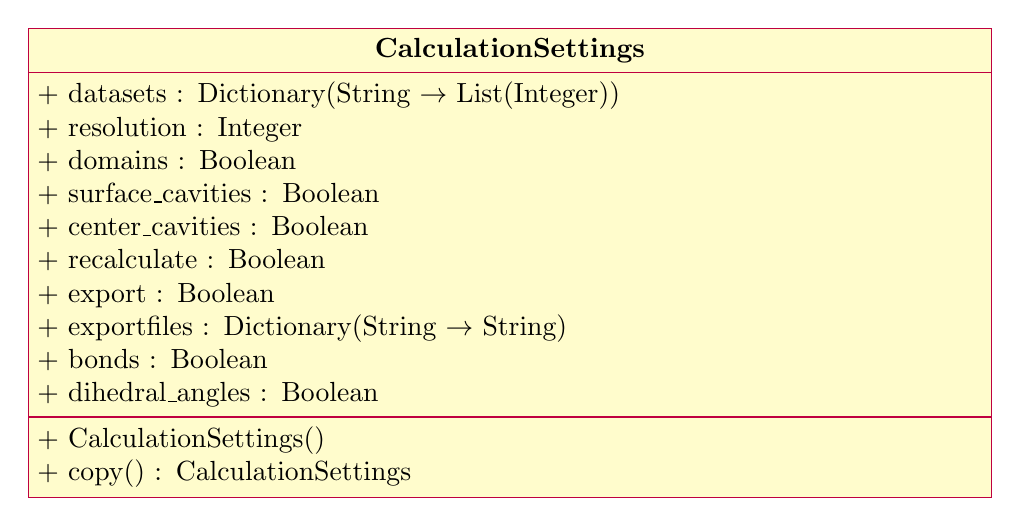
\begin{tikzpicture}
    \begin{class}[text width=\umlwidth]{CalculationSettings}{0, 0}
        \attribute{+ datasets : Dictionary(String $\rightarrow$ List(Integer))}
        \attribute{+ resolution : Integer}
        \attribute{+ domains : Boolean}
        \attribute{+ surface\_cavities : Boolean}
        \attribute{+ center\_cavities : Boolean}
        \attribute{+ recalculate : Boolean}
        \attribute{+ export : Boolean}
        \attribute{+ exportfiles : Dictionary(String $\rightarrow$ String)}
        \attribute{+ bonds : Boolean}
        \attribute{+ dihedral\_angles : Boolean}

        \operation{+ CalculationSettings()}
        \operation{+ copy() : CalculationSettings}
    \end{class}
\end{tikzpicture}

\noindent
The internal mechanism of caching and creating an index file:\\
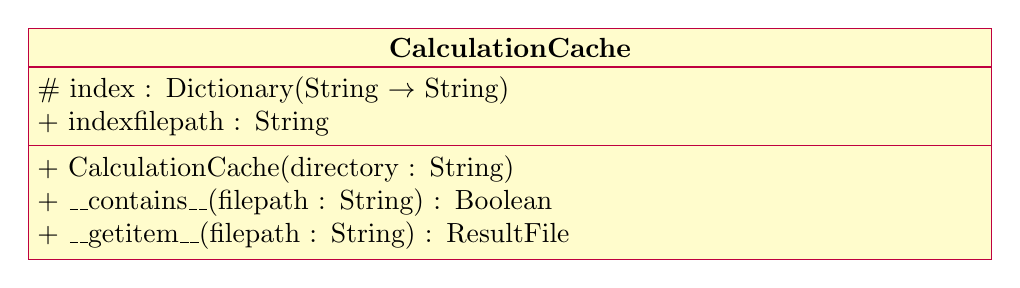
\begin{tikzpicture}
    \begin{class}[text width=\umlwidth]{CalculationCache}{0, 0}
        \attribute{\# index : Dictionary(String $\rightarrow$ String)}
        \attribute{+ indexfilepath : String}
        
        \operation{+ CalculationCache(directory : String)}
        \operation{+ \_\_contains\_\_(filepath : String) : Boolean}
        \operation{+ \_\_getitem\_\_(filepath : String) : ResultFile}
    \end{class}
\end{tikzpicture}

\subsection{Algorithm}
\todo{This part has not been refactored yet.}
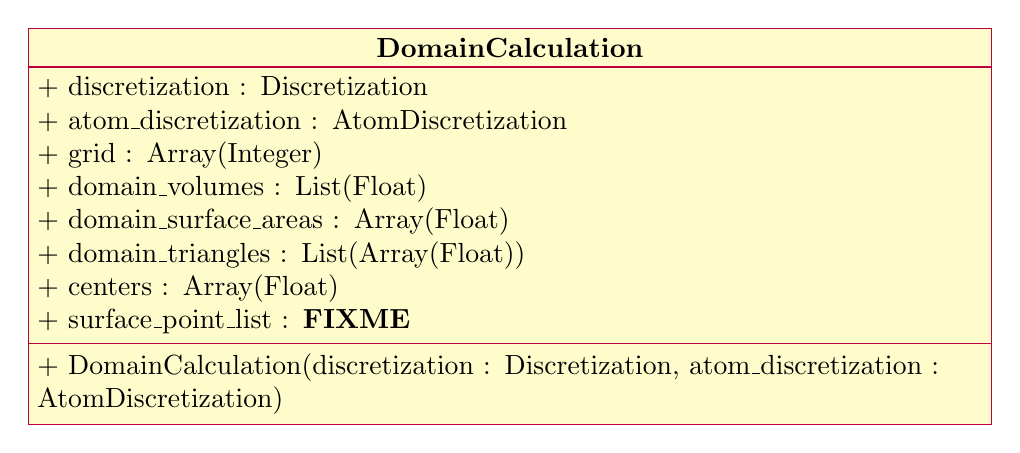
\begin{tikzpicture}
    \begin{class}[text width=\umlwidth]{DomainCalculation}{0, 0}
        \attribute{+ discretization : Discretization}
        \attribute{+ atom\_discretization : AtomDiscretization}
        \attribute{+ grid : Array(Integer)}
        \attribute{+ domain\_volumes : List(Float)}
        \attribute{+ domain\_surface\_areas : Array(Float)}
        \attribute{+ domain\_triangles : List(Array(Float))}
        \attribute{+ centers : Array(Float)}
        \attribute{+ surface\_point\_list : \textbf{FIXME}}
        
        \operation{+ DomainCalculation(discretization : Discretization, atom\_discretization : AtomDiscretization)}
    \end{class}
\end{tikzpicture}

\noindent
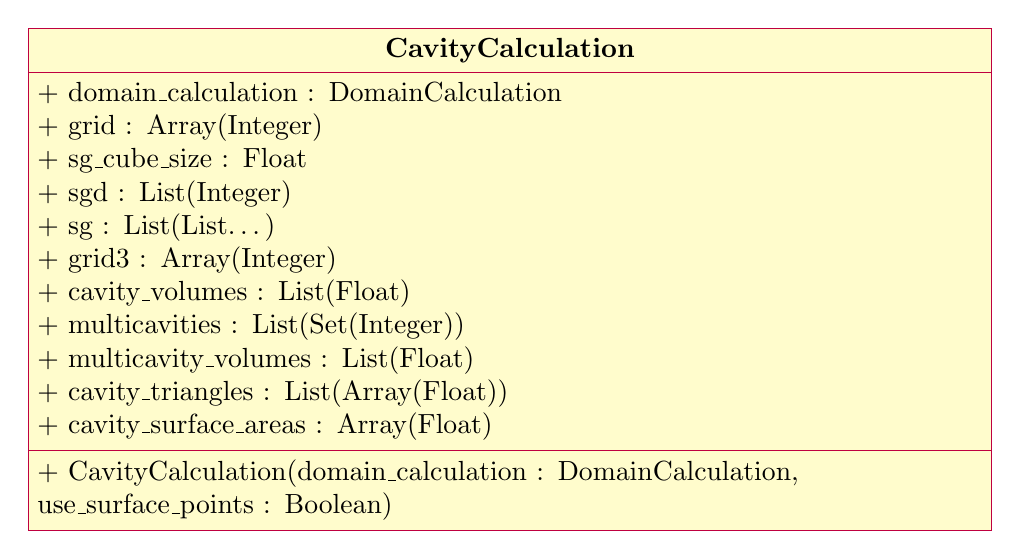
\begin{tikzpicture}
    \begin{class}[text width=\umlwidth]{CavityCalculation}{0, 0}
        \attribute{+ domain\_calculation : DomainCalculation}
        \attribute{+ grid : Array(Integer)}
        \attribute{+ sg\_cube\_size : Float}
        \attribute{+ sgd : List(Integer)}
        \attribute{+ sg : List(List\ldots)}
        \attribute{+ grid3 : Array(Integer)}
        \attribute{+ cavity\_volumes : List(Float)}
        \attribute{+ multicavities : List(Set(Integer))}
        \attribute{+ multicavity\_volumes : List(Float)}
        \attribute{+ cavity\_triangles : List(Array(Float))}
        \attribute{+ cavity\_surface\_areas : Array(Float)}
        
        \operation{+ CavityCalculation(domain\_calculation : DomainCalculation, use\_surface\_points : Boolean)}
    \end{class}
\end{tikzpicture}
\\\todo{Check what data types the code really produces}

\noindent
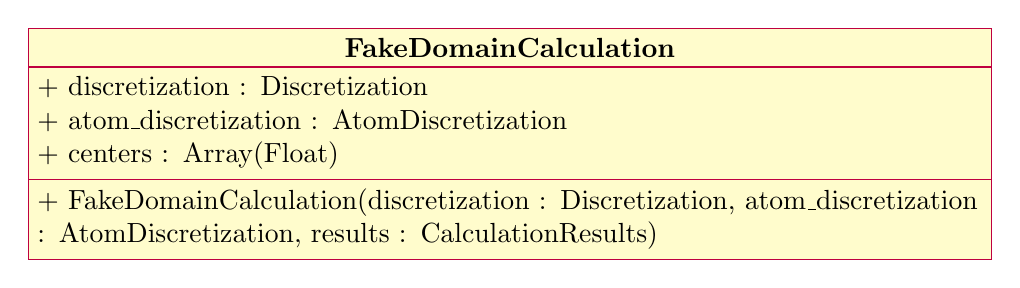
\begin{tikzpicture}
    \begin{class}[text width=\umlwidth]{FakeDomainCalculation}{0, 0}
        \attribute{+ discretization : Discretization}
        \attribute{+ atom\_discretization : AtomDiscretization}
        \attribute{+ centers : Array(Float)}

        \operation{+ FakeDomainCalculation(discretization : Discretization, atom\_discretization : AtomDiscretization, results : CalculationResults)}
    \end{class}
\end{tikzpicture}
\\\todo{\texttt{FakeDomainCalculation} uses the deprecated \texttt{CalculationResults}}



\end{document}
